\chapter{Data Definition}
\label{sec:data-definition}

This chapter describes the dataset used by \ldbcfinbench, including the data
schema design and the data generation process. Generally, we design
\ldbcfinbench balancing the reality and abstraction. There are some annotations
about the compromises in data design,
\begin{itemize}
    \item Although multiple persons/companies may own the same account in
          reality, an account is owned by a person or a company only in the
          schema to make it simple.
    \item Although rejected transactions may be recorded to support future loan
          decisions, only approved transactions/transfers are recorded in the
          benchmark dataset.
    \item Considering the DAU of financial systems in reality, There will be
          many signIn edges between medium and account vertices. However, we do
          not generate such many signIn edges aligning to reality with a limit
          in the simulation of data generation process since systems usually
          circumvent the problem by adding a medium attribute to edges like
          transfer and withdraw to record the medium users used.
\end{itemize}

\section{Data Types}

\autoref{table:types} describes the different data types used in the benchmark.
Compared with \ldbcsnb, there is a new compound type, \textbf{Path}, which is
widely applied in financial scenarios reflecting traces, e.g. fund transfer
traces. Note that the 32-bit floats used in \ldbcfinbench all round to 3 decimal
places(thousandths).

\begin{table}[h]
    \centering
    \begin{tabular}{|>{\typeCell}p{\attributeColumnWidth}|p{\largeDescriptionColumnWidth}|}
        \hline
        \tableHeaderFirst{Type} & \tableHeader{Description}                      \\
        \hline
        ID                      & Integer type with 64-bit precision. All IDs
        within a single entity type (e.g. Person) are unique, but different
        entity types (e.g. a Person and an Account) might have the same ID.      \\
        \hline
        32-bit Integer          & Integer type with 32-bit precision             \\
        \hline
        64-bit Integer          & Integer type with 64-bit precision             \\
        \hline
        32-bit Float            & Floating type with 32-bit precision
        \textbf{rounded to 3 decimal places(thousandths)}                        \\
        \hline
        String                  & Variable length text of size 40 Unicode
        characters                                                               \\
        \hline
        Long String             & Variable length text of size 256 Unicode
        characters                                                               \\
        \hline
        Text                    & Variable length text of size 2000 Unicode
        characters                                                               \\
        \hline
        Date                    & Date with a precision of a day, encoded as a
        string with the following format: \textit{yyyy-mm-dd}, where
        \textit{yyyy} is a four-digit integer representing the year, the year,
        \textit{mm} is a two-digit integer representing the month and
        \textit{dd} is a two-digit integer representing the day.                 \\
        \hline
        DateTime                & Date with a precision of milliseconds, encoded
        as a string with the following format:
        \textit{yyyy-mm-ddTHH:MM:ss.sss+0000}, where \textit{yyyy} is a
        four-digit integer representing the year, the year, \textit{mm} is a
        two-digit integer representing the month and \textit{dd} is a two-digit
        integer representing the day, \textit{HH} is a two-digit integer
        representing the hour, \textit{MM} is a two digit integer representing
        the minute and \textit{ss.sss} is a five digit fixed point real number
        representing the seconds up to millisecond precision. Finally, the
        \textit{+0000} of the end represents the timezone, which in this case is
        always GMT.                                                              \\
        \hline
        Boolean                 & A logical type taking the value of either True
        of False.                                                                \\
        \hline
        Enum                    & Enumeration type                               \\
        \hline
        Path                    & A compound type representing a trace which is
        expressed in an ordered sequence of vertices' IDs in the trace. For
        example, [1,3,4,8] expresses a trace 1->3->4->8.                         \\
        \hline
    \end{tabular}
    \caption{Description of the data types.}
    \label{table:types}
\end{table}

\subsection{Enumerations}
{\flushleft \textbf{TRUNCATION\_ORDER:}} The enumeration describes the sort
order before truncation. \textbf{TIMESTAMP\_ASCENDING} means truncation on
ascending order of timestamp.


\section{Data Schema}

\autoref{figure:schema} shows the data schema in UML. The schema defines the
structure of the data used in the benchmark in terms of entities and their
relations. Data represents a snapshot of the activity in several financial
scenarios during a period of time. The schema specifies different entities,
their attributes, and their relations. All of them are described in the
following sections.

\begin{figure}[htbp]
    \centering
    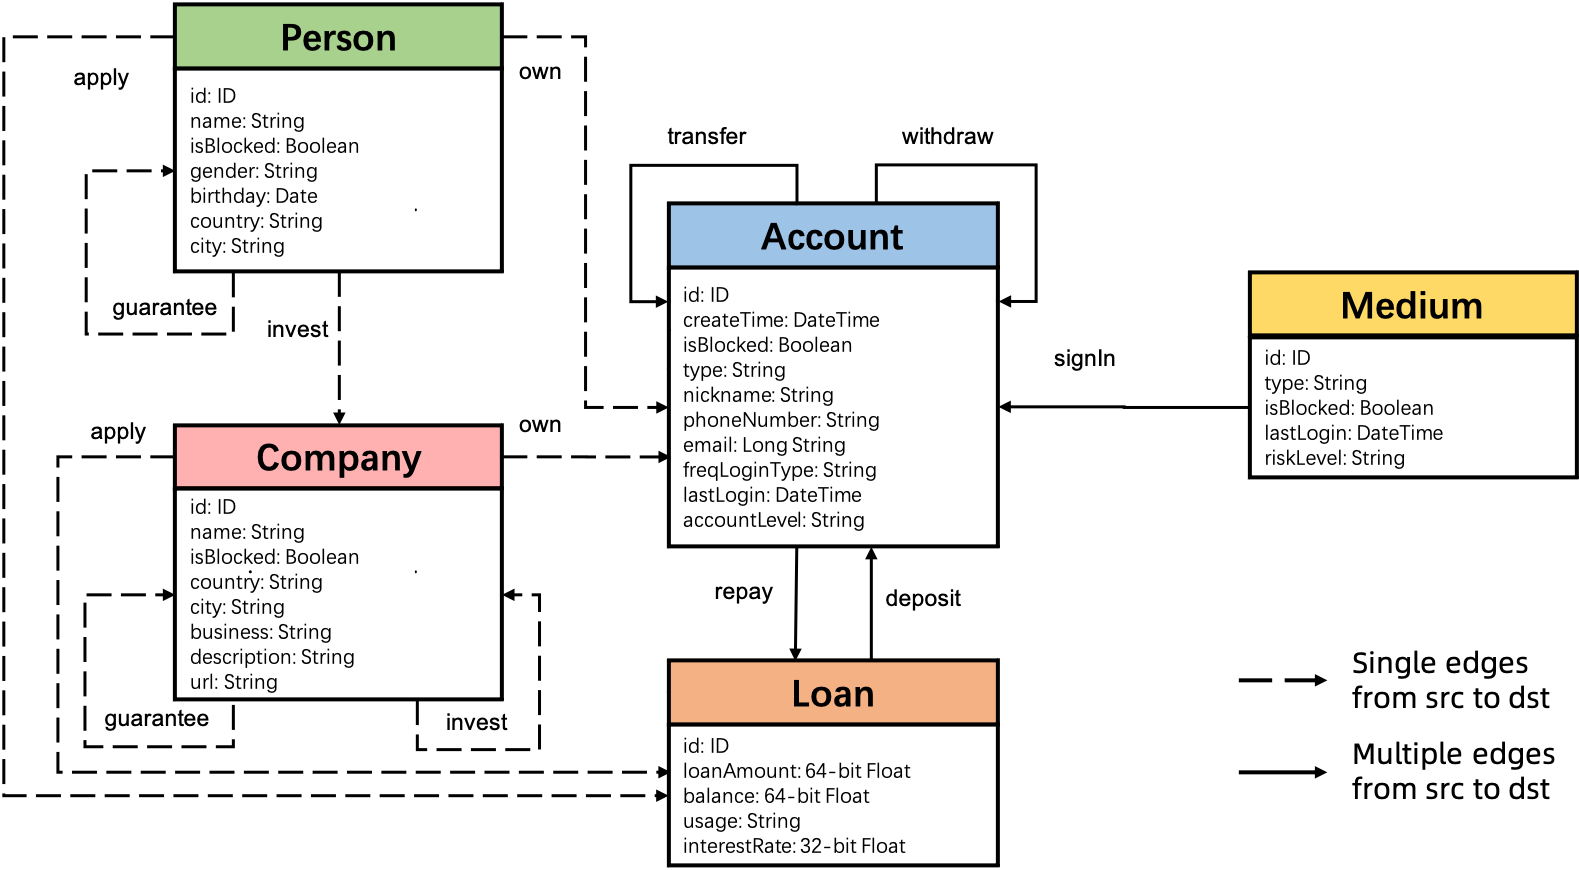
\includegraphics[width=\linewidth]{figures/data-schema}
    \caption{The \ldbcfinbench data schema}
    \label{figure:schema}
\end{figure}

\subsection{Entities}

{\flushleft \textbf{Person:}} A person of the real world. \autoref{table:person}
shows the attributes.
\begin{table}[H]
    \begin{tabular}{|>{\varNameCell}p{\attributeColumnWidth}|>{\typeCell}p{\typeColumnWidth}|p{\descriptionColumnWidth}|}
        \hline
        \tableHeaderFirst{Attribute} & \tableHeader{Type} &
        \tableHeader{Description}                                                         \\
        \hline
        id                           & ID                 & The identifier of the person. \\
        \hline
        name                         & String             & The name of the person.       \\
        \hline
    \end{tabular}
    \caption{Attributes of Person entity.}
    \label{table:person}
\end{table}

{\flushleft \textbf{Company:}} A company of the real world, which persons work
in and persons invest. \autoref{table:company} shows the attributes.
\begin{table}[H]
    \begin{tabular}{|>{\varNameCell}p{\attributeColumnWidth}|>{\typeCell}p{\typeColumnWidth}|p{\descriptionColumnWidth}|}
        \hline
        \tableHeaderFirst{Attribute} & \tableHeader{Type} &
        \tableHeader{Description}                                                          \\
        \hline
        id                           & ID                 & The identifier of the company. \\
        \hline
        name                         & String             & The name of the company.       \\
        \hline
    \end{tabular}
    \caption{Attributes of Company entity.}
    \label{table:company}
\end{table}

{\flushleft \textbf{Account:}} An account in real world financial systems, which
is registered and owned by persons and companies. It includes many types such as
personalDeposit, personalCredit, etc. It can deal with other accounts.
\autoref{table:account} shows the attributes.
\begin{table}[H]
    \begin{tabular}{|>{\varNameCell}p{\attributeColumnWidth}|>{\typeCell}p{\typeColumnWidth}|p{\descriptionColumnWidth}|}
        \hline
        \tableHeaderFirst{Attribute} & \tableHeader{Type} &
        \tableHeader{Description}                                                                              \\
        \hline
        id                           & ID                 & The identifier of the account.                     \\
        \hline
        createTime                   & DateTime           & The time when the account created.                 \\
        \hline
        isBlocked                    & Boolean            & If the account is blocked or concerned in systems. \\
        \hline
        type                         & String             & The type of Account including personalDeposit,
        personalCredit, companyDeposit, card.                                                                  \\
        \hline
    \end{tabular}
    \caption{Attributes of Account entity.}
    \label{table:account}
\end{table}

{\flushleft \textbf{Loan:}} A loan for persons and company to apply in real
world. \autoref{table:loan} shows the attributes.
\begin{table}[H]
    \begin{tabular}{|>{\varNameCell}p{\attributeColumnWidth}|>{\typeCell}p{\typeColumnWidth}|p{\descriptionColumnWidth}|}
        \hline
        \tableHeaderFirst{Attribute} & \tableHeader{Type} &
        \tableHeader{Description}                                                       \\
        \hline
        id                           & ID                 & The identifier of the loan. \\
        \hline
        loanAmount                   & 64-bit Integer     & The amount of a loan.       \\
        \hline
        balance                      & 64-bit Integer     & The balance of a loan.      \\
        \hline
    \end{tabular}
    \caption{Attributes of Loan entity.}
    \label{table:loan}
\end{table}

{\flushleft \textbf{Medium:}} An abstract standing for things that users use to
sign in account in real world, such as IP, mac, phone numbers.
\autoref{table:medium} shows the attributes.
\begin{table}[H]
    \begin{tabular}{|>{\varNameCell}p{\attributeColumnWidth}|>{\typeCell}p{\typeColumnWidth}|p{\descriptionColumnWidth}|}
        \hline
        \tableHeaderFirst{Attribute} & \tableHeader{Type} & \tableHeader{Description}                         \\
        \hline
        id                           & ID                 & The identifier of the medium.                     \\
        \hline
        type                         & String             & The medium type, e.g. POS, IP.                    \\
        \hline
        isBlocked                    & Boolean            & If the medium is blocked or concerned in systems. \\
        \hline
    \end{tabular}
    \caption{Attributes of Medium entity.}
    \label{table:medium}
\end{table}

\subsection{Relations}
Relations connect entities of different types showed in
\autoref{table:relations}. Except that own and workIn has no attributes, the
attributes of other relations are showed in the following tables. Note that the
Cardinality means the cardinal relationship from the tail to head of the edge
type and the Multiplicity means how many edges exist from the same tail to the
same head. For example, the 1 : N cardinality of own means an account can
only be owned by a person or a company.

\begin{longtable}{|>{\centering\varNameCell}p{1.5cm}|>{\typeCell}p{1.5cm}|>{\centering\cardinalCell}p{2cm}|>{\typeCell}p{1.5cm}|>{\centering\edgeDirectionCell}p{2cm}|p{5.5cm}|}
    \hline
    \tableHeaderFirst{Name} & \tableHeader{Tail}       & \tableHeader{Cardinality} & \tableHeader{Head}       & \tableHeader{Multiplicity} & \tableHeader{Description}                                            \\
    \hline
    signIn                  & Medium                   & N:N                       & Account                  & N                          & An account signed in with a media.                                   \\
    \hline
    own                     & Person/ \newline Company & 1:N                       & Account                  & 1                          & An account owned by a person or a company.                           \\
    \hline
    transfer                & Account                  & N:N                       & Account                  & N                          & Fund transferred between two accounts.                               \\
    \hline
    withdraw                & Account                  & N:N                       & Account                  & N                          & Fund transferred from an account to another account of type card.    \\
    \hline
    apply                   & Person/ \newline Company & 1:N                       & Loan                     & 1                          & A person or a company applies a Loan.                                \\
    \hline
    deposit                 & Loan                     & N:1                       & Account                  & N                          & Loan fund deposited to an account.                                   \\
    \hline
    repay                   & Account                  & 1:N                       & Loan                     & N                          & Loan repaid from an account.                                         \\
    \hline
    invest                  & Person/ \newline Company & N:N                       & Company                  & 1                          & A person or a company invests a company.                             \\
    \hline
    workIn                  & Person                   & N:N                       & Company                  & 1                          & A person works in a company.                                         \\
    \hline
    guarantee               & Person/ \newline Company & N:N                       & Person/ \newline Company & 1                          & A person or a company guarantees another for some reason like loans. \\
    \hline
    \caption{Description of the data relations.}
    \label{table:relations}
\end{longtable}

{\flushleft \textbf{transfer:}} Fund transfers between accounts. \autoref{table:transfer} shows the attributes.
\begin{table}[H]
    \begin{tabular}{|>{\varNameCell}p{\attributeColumnWidth}|>{\typeCell}p{\typeColumnWidth}|p{\descriptionColumnWidth}|}
        \hline
        \tableHeaderFirst{Attribute} & \tableHeader{Type} & \tableHeader{Description}      \\
        \hline
        timestamp                    & DateTime           & The time when transfer issues. \\
        \hline
        amount                       & 64-bit Integer     & The amount of the transfer.    \\
        \hline
        type                         & String             & The type of the transfer.      \\
        \hline
    \end{tabular}
    \caption{Attributes of transfer relation.}
    \label{table:transfer}
\end{table}

{\flushleft \textbf{withdraw:}} Fund is transferred from an account to another of type card. \autoref{table:withdraw} shows the attributes.
\begin{table}[H]
    \begin{tabular}{|>{\varNameCell}p{\attributeColumnWidth}|>{\typeCell}p{\typeColumnWidth}|p{\descriptionColumnWidth}|}
        \hline
        \tableHeaderFirst{Attribute} & \tableHeader{Type} & \tableHeader{Description}      \\
        \hline
        timestamp                    & DateTime           & The time when withdraw issues. \\
        \hline
        amount                       & 64-bit Integer     & The amount of the withdraw.    \\
        \hline
    \end{tabular}
    \caption{Attributes of withdraw relation.}
    \label{table:withdraw}
\end{table}

{\flushleft \textbf{repay:}} Loan is repaid from an account. \autoref{table:repay} shows the attributes.
\begin{table}[H]
    \begin{tabular}{|>{\varNameCell}p{\attributeColumnWidth}|>{\typeCell}p{\typeColumnWidth}|p{\descriptionColumnWidth}|}
        \hline
        \tableHeaderFirst{Attribute} & \tableHeader{Type} & \tableHeader{Description}   \\
        \hline
        timestamp                    & DateTime           & The time when repay issues. \\
        \hline
        amount                       & 64-bit Integer     & The amount of the repay.    \\
        \hline
    \end{tabular}
    \caption{Attributes of repay relation.}
    \label{table:repay}
\end{table}

{\flushleft \textbf{deposit:}} Loan fund is deposited to an account. \autoref{table:deposit} shows the attributes.
\begin{table}[H]
    \begin{tabular}{|>{\varNameCell}p{\attributeColumnWidth}|>{\typeCell}p{\typeColumnWidth}|p{\descriptionColumnWidth}|}
        \hline
        \tableHeaderFirst{Attribute} & \tableHeader{Type} & \tableHeader{Description}     \\
        \hline
        timestamp                    & DateTime           & The time when deposit issues. \\
        \hline
        amount                       & 64-bit Integer     & The amount of the deposit.    \\
        \hline
    \end{tabular}
    \caption{Attributes of deposit relation.}
    \label{table:deposit}
\end{table}

{\flushleft \textbf{signIn:}} An account is signed in with a Media. \autoref{table:signIn} shows the attributes.
\begin{table}[H]
    \begin{tabular}{|>{\varNameCell}p{\attributeColumnWidth}|>{\typeCell}p{\typeColumnWidth}|p{\descriptionColumnWidth}|}
        \hline
        \tableHeaderFirst{Attribute} & \tableHeader{Type} & \tableHeader{Description}     \\
        \hline
        timestamp                    & DateTime           & The time when signIn happens. \\
        \hline
    \end{tabular}
    \caption{Attributes of signIn relation.}
    \label{table:signIn}
\end{table}

{\flushleft \textbf{invest:}} A person or a company invests a company. \autoref{table:invest} shows the attributes.
\begin{table}[H]
    \begin{tabular}{|>{\varNameCell}p{\attributeColumnWidth}|>{\typeCell}p{\typeColumnWidth}|p{\descriptionColumnWidth}|}
        \hline
        \tableHeaderFirst{Attribute} & \tableHeader{Type} & \tableHeader{Description}     \\
        \hline
        timestamp                    & DateTime           & The time when invest happens. \\
        \hline
        ratio                        & 32-bit Float       & The ratio of the investment.  \\
        \hline
    \end{tabular}
    \caption{Attributes of invest relation.}
    \label{table:invest}
\end{table}

{\flushleft \textbf{apply:}} A person or a company applies a Loan. \autoref{table:apply} shows the attributes.
\begin{table}[H]
    \begin{tabular}{|>{\varNameCell}p{\attributeColumnWidth}|>{\typeCell}p{\typeColumnWidth}|p{\descriptionColumnWidth}|}
        \hline
        \tableHeaderFirst{Attribute} & \tableHeader{Type} & \tableHeader{Description}    \\
        \hline
        timestamp                    & DateTime           & The time when apply happens. \\
        \hline
    \end{tabular}
    \caption{Attributes of apply relation.}
    \label{table:apply}
\end{table}

{\flushleft \textbf{guarantee:}} A person or a company guarantees another for some reason like Loans. \autoref{table:guarantee} shows the attributes.
\begin{table}[H]
    \begin{tabular}{|>{\varNameCell}p{\attributeColumnWidth}|>{\typeCell}p{\typeColumnWidth}|p{\descriptionColumnWidth}|}
        \hline
        \tableHeaderFirst{Attribute} & \tableHeader{Type} & \tableHeader{Description}        \\
        \hline
        timestamp                    & DateTime           & The time when guarantee happens. \\
        \hline
    \end{tabular}
    \caption{Attributes of guarantee relation.}
    \label{table:guarantee}
\end{table}

\section{Data Generation}
 [TODO. This section will be filled after benchmark software designed and developed.]

\section{Output Data}
 [TODO. This section will be filled after benchmark software designed and developed.]\